\section{Verification and performance evidence}
\label{sec:experiments}

The archive separates correctness tests, deterministic work counters, and
timing experiments.  None can replace the others.  Exhaustive finite tests
are particularly useful for gluing and parity conventions; the theorems
establish the general claims.  Operation counts expose structural work;
wall-clock ratios determine whether the Python implementation benefits on
the tested machine.

\subsection{Independent correctness checks}

\begin{table}[htbp]
\centering\small
\begin{tabular}{P{34mm}P{108mm}}
\toprule
Component & Verification performed \\
\midrule
Interlacement discovery & All 146,600 canonical double-occurrence words
through seven labels, compared with an explicit interlacement graph;
separate forest and separation certificate verification. \\
PD factor reconstruction & 32,055 rotation assignments through five
crossings, of which 2,109 validate as spherical; 600 generated braid knots,
600 relabelings, and 14 supplied fixtures.  All 3,323 validated diagrams
have the same factor PD multiset as the archived geometric algorithm. \\
Sparse determinant & 450 small matrices against the independent Leibniz
formula; 420 additional dense comparisons; permutation matrices through
dimension 1,000; singularity, input preservation, complete-pivot signs,
resource callbacks, and transient nonzero-count regression. \\
Pointed algebra & Lift--compose--quotient identities for every polynomial
input on all triples of noncrossing matchings through six endpoints. \\
Pointed diagram scan & 2,898 signed braid diagrams against an independent
dense reduced-cube oracle; 8,002 rank scans, including 5,052 additional
basepoint/order variations; 2,898 decision scans; 42 cache pairs;
intermediate differential-square checks. \\
Frontier correction & Exact enumeration of full prefix resolutions,
independent component counting and Laurent coefficients; agreement with
both reference and optimized gluing engines. \\
Hierarchy budget & All 364 radix tuples of length at most five with
radices in $\{1,2,3\}$; 284,932 strict transitions; 17,021 explicit
decreasing sequences in the smallest cases. \\
\bottomrule
\end{tabular}
\caption{Finite verification supporting distinct parts of the research.
The sets of scans overlap as described; their counts are not counts of
distinct knot types.}
\label{tab:validation}
\end{table}

The two main algebraic crosschecks use separate constructions.  Factor
discovery is checked against an explicit graph, and its PD output against
the archived face-based algorithm.  The pointed scanner is checked against
a dense cube construction, not merely against its own unpointed quotient
code.  The baseline's division by two in each homological degree is justified
by the characteristic-two splitting, which changes quantum degree only
\cite[Corollary~3.2.C]{shumakovitch2014}.

The complete regression suite also retains the original tests.  New
integration checks cover budget exceptions during factorization, propagation
to \code{UNKNOWN}, evidence compatibility, and exact transient sparse
storage counters.  The final executable test log is retained in
\path{data/unit_tests.txt}.  These are finite validation results, not a
formal proof-assistant verification of the Python interpreter or the whole
topological theory.

\subsection{Measurement protocol}

Measurements use Python 3.12.14 on the supplied x86-64 Linux environment.
The archive records the platform string, seeds, source hashes where captured,
input generators, raw times, crossing orders, work counters, and A/A controls.
It does not claim CPU isolation, fixed frequency, or performance portability.
The considerable variability in some small A/A cases precludes a persuasive
claim about changes of only a few percent on those cases.

For factorization, sparse elimination, and the full pipeline, each block
randomly orders two baseline calls and two updated calls.  Inputs are
preconstructed; timed calls receive fresh diagram objects to prevent cached
diagram properties from moving between arms.  Some fast cases use a common
small batch count.  The block ratio is the arithmetic mean of the two updated
times divided by the arithmetic mean of the two baseline times.  Nine blocks
give the displayed median ratio.  Under an independent-block interpretation,
the interval from the second to the eighth ordered ratio has nominal
coverage $1-2(1+9)/2^9=0.9609375$ for the population median.  Dependence and
shared-environment drift are not removed by this calculation.

The separate pointed experiment uses the same precomputed crossing order
for both engines and randomizes two calls of each per block.  Its block
ratio is the ratio of the \emph{geometric} means, and its intervals are
percentile bootstrap intervals for the median, using 2,000 resamples.
It uses 51 blocks for small cases and 21 for the stress closure.  The two
experiments' interval methods are explicitly different; they should not be
treated as identical estimators.

Pooled arm medians in milliseconds provide a readable scale.  Their quotient
need not equal the median paired ratio, because median and division do not
commute.  Ratios below one favor the updated implementation.  Intervals
describe measurement uncertainty for these fixed inputs, not uncertainty
about an asymptotic theorem or a representative distribution of all knots.

The final audit changed the sparse peak counter and recognition's budget
handling.  Sparse and pipeline timings were therefore repeated on that final
code.  The earlier factorization algorithm was unchanged and retains its
original paired measurements.  The first pointed timing used a development
wrapper; it too was repeated against the final public API.  Both earlier
and final raw records remain in the archive, with their provenance.

\subsection{Visible factorization and complete-pipeline gains}

\begin{table}[htbp]
\centering\small
\begin{tabular}{lrrrrl}
\toprule
Summands & $n$ & Baseline ms & Updated ms & Ratio & 96.1\% interval \\
\midrule
8 & 24 & 2.652 & 0.280 & 0.127 & [0.0880, 0.346] \\
32 & 96 & 23.013 & 1.242 & 0.0645 & [0.0397, 0.0987] \\
128 & 384 & 372.151 & 5.565 & 0.0162 & [0.0135, 0.0205] \\
256 & 768 & 1328.586 & 9.479 & 0.00687 & [0.00606, 0.00956] \\
512 & 1536 & 5602.400 & 23.656 & 0.00405 & [0.00368, 0.00459] \\
\bottomrule
\end{tabular}

\caption{Checked factorization of the specified cyclic trefoil sums.
The input diagram is already constructed, but output factor validation
is timed.  This compares with the quadratic-work embedding proved in
Theorem~\ref{thm:quadratic-factor-family}.}
\label{tab:factor-times}
\end{table}

The largest factorization example has 512 summands and 1,536 crossings.
Its old recursive calls collectively visit 393,981 crossings before leaf
work, whereas the new algorithm discovers the component partition in one
pass and reconstructs all factors together.  The measured difference is
consistent with that structural change.  It is not needed to prove the
quadratic lower bound or the new upper bound.

\begin{table}[htbp]
\centering\small
\begin{tabular}{lrrrrl}
\toprule
Diagram & $n$ & Baseline ms & Updated ms & Ratio & 96.1\% interval \\
\midrule
Conway & 11 & 1.139 & 1.304 & 1.288 & [0.459, 2.185] \\
Hard unknot (8) & 8 & 0.839 & 0.757 & 0.901 & [0.622, 1.082] \\
Kinoshita--Terasaka & 11 & 1.483 & 1.315 & 0.848 & [0.690, 1.286] \\
128 trefoils & 384 & 355.975 & 8.024 & 0.0223 & [0.0214, 0.0259] \\
256 trefoils & 768 & 1347.937 & 12.440 & 0.00980 & [0.00751, 0.0102] \\
$T(3,521)$ & 1042 & 181.906 & 47.122 & 0.263 & [0.236, 0.269] \\
\bottomrule
\end{tabular}

\caption{Complete recognition with the updated defaults and the archived
defaults.  The pointed option is off in this comparison.}
\label{tab:pipeline-times}
\end{table}

The whole-pipeline comparison shows that the factorization benefit survives
integration.  On connected sums, the pipeline no longer pays repeated global
reconstruction before examining its first decisive summand.  The large torus
example also benefits from the sparse filter.  The small Conway,
Kinoshita--Terasaka, and hard-unknot fixtures show no consistent substantial
improvement; their noisy results are included to avoid generalizing the
large-family gains to every use case.

\subsection{Sparse elimination: measured work and crossover}

\begin{table}[htbp]
\centering\small
\begin{tabular}{lrrrrl}
\toprule
Diagram & $n$ & Baseline ms & Updated ms & Ratio & 96.1\% interval \\
\midrule
$T(3,31)$ & 62 & 1.352 & 1.792 & 1.431 & [1.021, 1.716] \\
$T(3,127)$ & 254 & 7.520 & 7.033 & 0.958 & [0.793, 0.994] \\
$T(3,257)$ & 514 & 32.156 & 13.778 & 0.415 & [0.361, 0.476] \\
$T(3,521)$ & 1042 & 116.874 & 26.867 & 0.223 & [0.219, 0.232] \\
$T(3,1031)$ & 2062 & 529.732 & 59.900 & 0.115 & [0.108, 0.128] \\
\bottomrule
\end{tabular}

\caption{The original dense modular Alexander filter versus a forced
sparse backend on $T(3,q)$ diagrams with $n=2q$.  Forced sparse results
below the default 256-crossing threshold are retained.}
\label{tab:alexander-times}
\end{table}

\begin{table}[htbp]
\centering\small
\begin{tabular}{rrrrrr}
\toprule
$n$ & $E$ (per minor) & $F_{-1}$ & $F_t$ & $Z_{\max,-1}$ & $Z_{\max,t}$ \\
\midrule
62 & 180 & 109 & 170 & 180 & 180 \\
254 & 756 & 461 & 746 & 756 & 756 \\
514 & 1536 & 937 & 1526 & 1536 & 1536 \\
1042 & 3120 & 1905 & 3110 & 3120 & 3120 \\
2062 & 6180 & 3775 & 6170 & 6180 & 6180 \\
\bottomrule
\end{tabular}

\caption{Deterministic sparse counters for the two evaluated minors.
$F$ counts all attempted Schur positions.  $Z_{\max}$ includes transient
nonzeros inside a row update in the final implementation.}
\label{tab:sparse-work}
\end{table}

The sampled matrices maintain small pivot neighborhoods, so the counter
$F$ is far below a cubic dense-matrix allowance.  At the small end, incidence
and priority management can outweigh this saving.  This motivates an
explicit crossover policy and supports keeping both backends available.
The observations do not prove a fill theorem for the torus family or for
general Alexander matrices; such a theorem is a separate research question.

\begin{figure}[htbp]
\centering
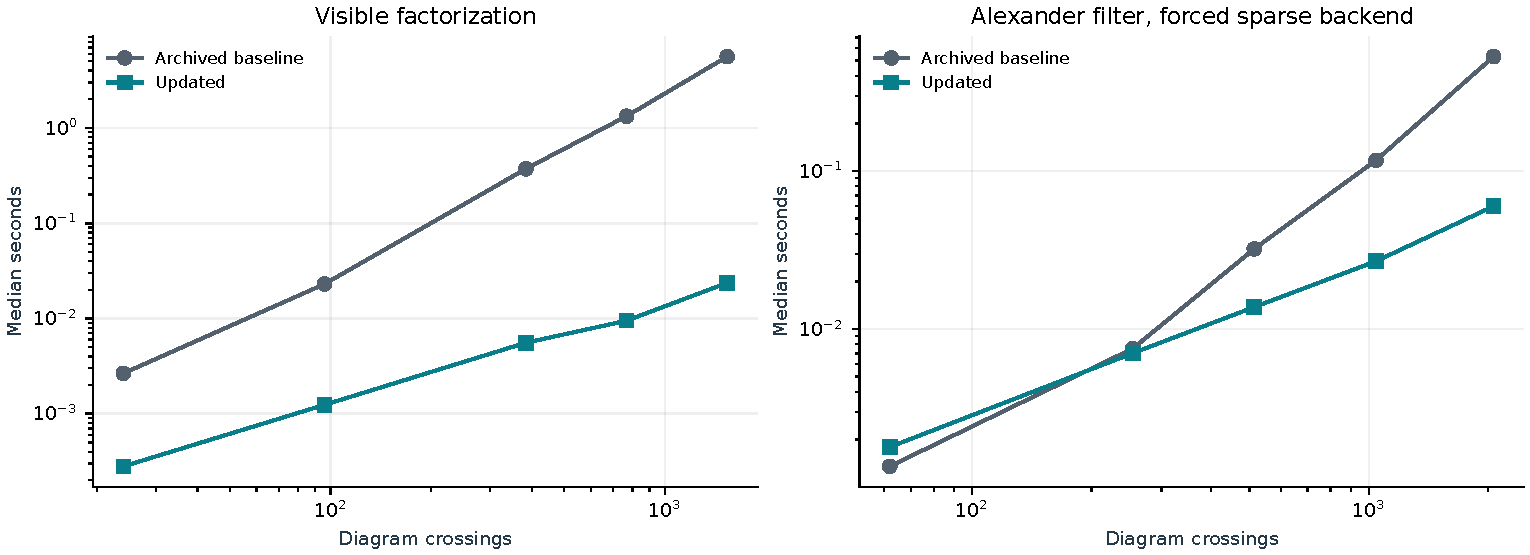
\includegraphics[width=\linewidth]{figures/scaling.pdf}
\caption{Measured scaling on two specified families.  Lines connect sampled
input sizes and are not fitted asymptotic exponents.  The factorization
comparison also has a structural proof; the sparse-family comparison has
a bound in terms of elimination work and measured pivot counters.}
\label{fig:scaling}
\end{figure}

\subsection{Pointed scanning: savings and regressions}

\begin{table}[htbp]
\centering\small
\begin{tabular}{lrrrl}
\toprule
Diagram & $n$ & Baseline ms & Pointed ms & Ratio [95\% bootstrap interval] \\
\midrule
Conway & 11 & 7.671 & 7.762 & 1.046 [0.939, 1.125] \\
Kinoshita--Terasaka & 11 & 6.905 & 7.090 & 1.004 [0.966, 1.069] \\
Hard unknot (8) & 8 & 1.168 & 1.268 & 1.191 [1.015, 1.275] \\
Unknot braid (40) & 40 & 1.683 & 1.948 & 1.114 [1.045, 1.231] \\
Stress closure (36) & 36 & 506.808 & 381.397 & 0.723 [0.673, 0.780] \\
$T(3,11)$ & 22 & 8.225 & 9.300 & 1.119 [1.072, 1.158] \\
Survivor 0 & 16 & 9.382 & 8.597 & 0.921 [0.896, 0.969] \\
Survivor 1 & 15 & 10.704 & 11.902 & 1.054 [1.021, 1.126] \\
Survivor 2 & 15 & 5.453 & 5.728 & 1.094 [1.007, 1.231] \\
\bottomrule
\end{tabular}

\caption{Direct reduced versus ordinary full-rank scanning, with the same
precomputed order.  These timings exclude the recognizer's preceding
filters and do not time early termination.}
\label{tab:pointed-times}
\end{table}

\begin{table}[htbp]
\centering\small
\begin{tabular}{lrrrr}
\toprule
Diagram & Compositions A & Compositions B & Peak objects A & Peak objects B \\
\midrule
Conway & 90 & 56 & 246 & 123 \\
Hard unknot (8) & 0 & 0 & 11 & 11 \\
Stress closure (36) & 23710 & 16705 & 17694 & 12341 \\
$T(3,11)$ & 214 & 75 & 126 & 77 \\
\bottomrule
\end{tabular}

\caption{Selected deterministic scanner counters.  A is the ordinary
scanner; B is the pointed scanner.  Peak objects are measured before
cancellation at each crossing.}
\label{tab:pointed-work}
\end{table}

On the 36-crossing stress closure, compositions decrease from 23,710 to
16,705, peak objects from 17,694 to 12,341, and transferred entries from
251,455 to 173,583.  These are exact work-count changes for the specified
order.  They do not amount to halving the whole computation, and the
timing table confirms that the effect depends on the input.

The three survivor cases are simplified unknot diagrams retained by the
repository's hard-unknot experiment after its filters fail to decide.
They are relevant to the residual decision stage, but have only 15 or 16
crossings.  Their results must not be extrapolated to large difficult
unknots.  The stress closure is useful for measuring substantial homological
work; it is not evidence that the complete pipeline needs homology on
every large input.

\begin{figure}[htbp]
\centering
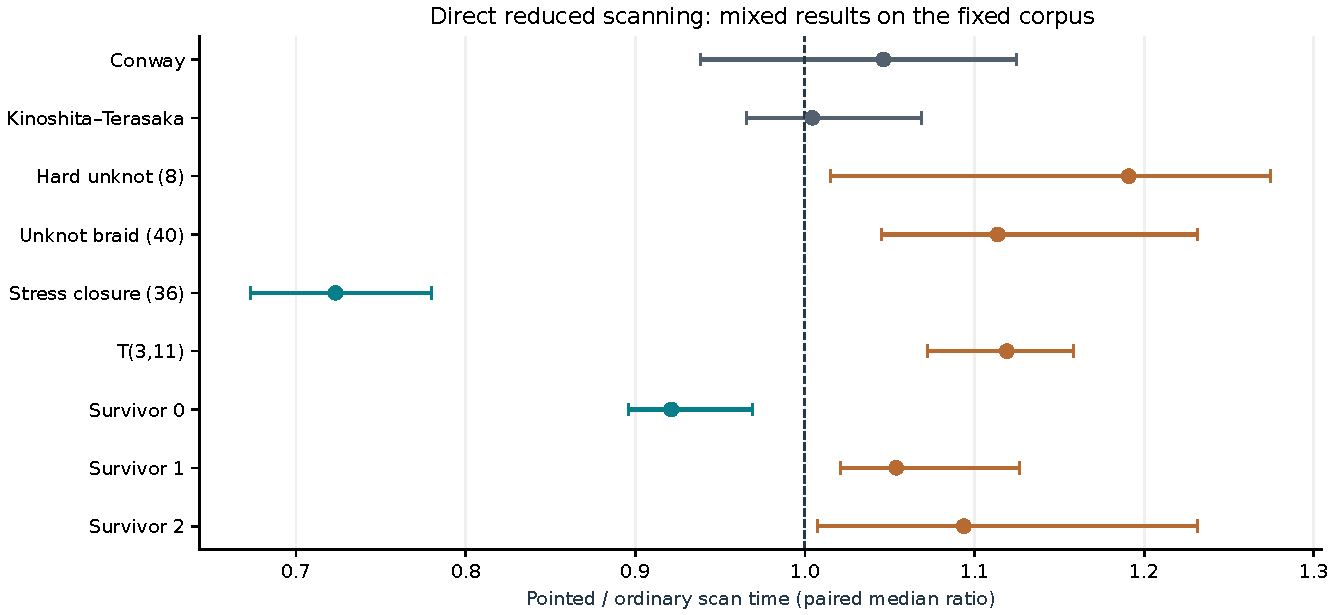
\includegraphics[width=\linewidth]{figures/pointed_ratios.pdf}
\caption{Pointed scan ratios with nominal 95\% bootstrap intervals.
The vertical reference is equal time.  Mixed results support retaining
an explicit \code{--pointed} option instead of changing the default scan.}
\label{fig:pointed-ratios}
\end{figure}

The before-closure examples in Section~\ref{sec:pointed} validate a new
decision mechanism.  They are not added to a headline speedup figure,
because visible factorization already handles those connected sums.  An
honest next experiment should seek prime-looking filter survivors on which
the certificate arises substantially before the last crossing.

\subsection{What the experiment does not settle}

The corpus contains deterministic constructed families and small finite
enumerations.  It is neither a uniform sample of knot types nor a validated
distribution of hard unknot instances.  Relabeled diagrams improve
representation coverage without adding knot types.  Exhaustive braid-word
enumeration similarly contains repeated knots.  Large filter-decided examples
mainly test preprocessing and rejection; a general complexity claim must
also handle large unknots and nontrivial knots that survive all filters.

The remaining quantitative uncertainty is explicit: there is no universal
bound on retained multiplicity, no guarantee of a useful early isolated
summand, no implemented noose certificate for the current order, and no
constructive hierarchy backend satisfying Section~\ref{sec:hierarchy}.
The experiments measure completed changes while leaving these obligations
open.
